
\subsection{Дз 1}

\vspace{5pt} <<\indef{Ботинки-2}>>. Есть $n$ игроков, каждый из которых владеет левым ботинком, и есть еще $m$ игроков, каждый из которых владеет правым ботинком, $n>m$. Каждый левый подходит к каждому правому. Одна полная пара ботинок стоит 1 рубль.  

Найдите ядро;

Найдите вектор Шепли для $n=3$ и $m=2$;

В изначальной постановке спрашивался вектор Шепли для произвольного $n$ и $m$\footnote{Мне почему-то показалось, что очевидным будет ответ типа $n/(n+m)$. Это ошибка.}. В явном виде (без громоздкой суммы) этот вектор не находится. Предложите какую-нибудь аппроксимацию для больших $n$ и $m$ с помощью нормального распределения;

\vspace{5pt} <<\indef{Гномы и золото}>>. Группа из $n$ гномов нашла много золотых слитков в пещере. Начинается обвал, поэтому нужно срочно убегать из пещеры. После обвала пещера окажется недоступной. Слитки золота тяжелы: в одиночку ни один гном не может нести слиток, но два гнома могут свободно нести один слиток. Снаружи пещеры слитки золота можно продать по цене 1 рубль за штуку. 
\begin{itemize}
\item Найдите ядро и вектор Шепли для произвольного $n$
\item Прокомментируйте разницу для четного и нечетного $n$
\end{itemize}

Ищем вектор Шепли для $n\geq 2$. Все гномы одинаковые, значит и получают одинаково. Общий доход равен $k$ если гномов $2k$ или $2k+1$. Соответственно, вектор Шепли - это $(0.5,0.5,...)$ для четного $n$ и $(\frac{k}{2k+1},\frac{k}{2k+1},...)$ для $n=2k+1$.

Ищем ядро. Если $n=2$, то ядро это все векторы вида $x_{1}+x_{2}=1$. Рассмотрим случай $n=2k+1>2$. Сумма выигрышей любых $2k$ гномов должна быть больше либо равна $k$, т.е. $x_{1}+x_{2}+...+x_{n}-x_{i}\geq k$ для всех $i$ (без любого гнома можно обойтись). Сложим все $2k+1$ неравенство, получим, что $2k\cdot (x_{1}+x_{2}+...x_{n})\geq (2k+1)k$. С другой стороны $x_{1}+x_{2}+...+x_{n}\leq k$. Противоречие, ядро пусто. Возьмем случай $n=2k>2$. Пусть какому-нибудь гному обещают меньше $v<1/2$. Поскольку любые два гнома могут заработать $1$, то из этого следует, что все остальные гномы должны получать как минимум $1-v>1/2$. Тогда суммарный заработок будет больше $k$, что невозможно. Значит все гномы получают минимум по $1/2$. А больше  - нет денег. Поэтому при $n=2k$ ядро совпадает с вектором Шепли.

Мораль: вектор Шепли старается делить <<по справедливости>>, т.е. если игроки одинаковые, значит всем поровну. А ядро проверяет <<устойчивость>> дележа. Когда гномов $2k+1$ один гном оказывается не при делах, и он готов на любую уступку, <<да я даже за одну копейку готов нести!>>. И этот гном без ноши мешает договорам других.


\vspace{5pt} <<\indef{Угадай цену пирога}>>
От пирога остался один кусочек\footnote{Эта игра реально играется в Голландии в семьях при дележе чего-нибудь между детьми. И на разных шоу, конечно.}. На него претендуют три брата. Папа предлагает им по очереди попробовать угадать цену пирога: сначала гадает старший, затем - средний и в конце - младший. Братья знают, что цены пирогов распределены равномерно на $[0;1]$. тот из братьев, чья версия ближе всего к правильной, получает пирог.

Найдите ядро и вектор Шепли в кооперативном варианте игры;


Найдите равновесие по Нэшу, совершенное в подыграх в некооперативном варианте игры;


Прокомментируйте;

\vspace{5pt} <<\indef{Помещик и крестьяне}>>
Есть один помещик и $n$ крестьян. Помещик владеет полем. Без поля крестьяне не могут ничего заработать. Если помещик предоставил поле и на нем работают $k$ крестьян, то они получают выгоду $f(k)$, где $f$ - функция с $f'>0$. 

Найдите ядро и вектор Шепли

Предложите примерное геометрическое описание для выигрыша помещика


\vspace{5pt} <<\indef{3 player unanimity game}>>
Илья Муромец, Алеша Попович и Добрыня Никитич охотятся на Змеев-Горынычей. В одиночку никто из них не может одолеть ни одного Змея-Горыныча. Втроем - могут одолеть одного Змея-Горыныча за час, вдвоем - $\alpha\in (0;1)$ Змеев-Горынычей за час.

Найдите ядро и вектор Шепли для произвольного $\alpha$

\vspace{5pt} <<\indef{Малое Гадюкино}>>
От шоссе до деревни Малое Гадюкино идет грунтовая дорога. Осенью дорога приходит в ужасное состояние, поэтому Малые Гадюкинцы на общем собрании решили заасфальтировать ее. При распределении затрат необходимо учесть тот факт, что деревня растянута вдоль дороги, и фактически Гадюкинцы живут на разных расстояниях от шоссе. Всего в Малом Гадюкино обитает  $n$  семей, на расстояниях от шоссе равных  $x_{1}$,  $x_{2}$,...  $x_{n}$ метров. За 1 рубль можно заасфальтировать 1 метр.


%\begin{figure}
%\centering
%\begin{asy}
%import unicode;
%texpreamble("\usepackage{mathtext}\usepackage[russian]{babel}");
%defaultpen(font("T2A","cmr","m","n"));
%unitsize (1cm);
%
%/* Рисуем Шоссе */
%draw ((0,-1)--(0,1),linewidth(4)); 
%
%draw ((0,0)--(9,0)); 
%
%
%dot ((4,0)); 
%label("$x_{1}$",(4,0),S); 
%
%dot ((5,0)); 
%label("$x_{2}$",(5,0),S); 
% 
%dot ((7,0));  
%label("...",(7,0),S); 

%dot ((9,0));  
%label("$x_{n}$",(9,0),S); 


%draw((2,-1.5)--(0.2,-1.2),Arrow); 
%label("\begin{small}Шоссе\end{small}",(2,-1.5),E); 

%draw((3,0.7)--(2,0.2),Arrow); 
%label("\begin{small}Грунтовая дорога\end{small}",(3,0.7),E); 


%\end{asy}

%\caption{Embedded Asymptote figures are easy!}
%\label{fig:embedded}
%\end{figure}

\begin{figure}[htbp]
	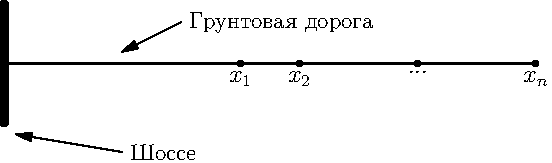
\includegraphics{coop_gadukino.pdf}
\end{figure}





Найдите вектор Шепли.

\vspace{5pt} <<\indef{Нефтепровод}>>

Нефть можно доставить из точки А в точку Б по нефтепроводу. 

%\begin{figure}[htbp]
%\begin{asy}
%
%import unicode;
%texpreamble("\usepackage{mathtext}\usepackage[russian]{babel}");
%defaultpen(font("T2A","cmr","m","n"));
%unitsize (1cm);

%draw("\begin{small}4\end{small}",(0,0)--(1,-1),Arrow);
%draw("\begin{small}1\end{small}",(0,0)--(1,1),S,Arrow);
%draw("\begin{small}3\end{small}",(1,1)--(1,-1),Arrow);
%draw("\begin{small}2\end{small}",(1,1)--(2,0),S,Arrow);
%draw("\begin{small}5\end{small}",(1,-1)--(2,0),Arrow);
%
%dot((0,0));
%label("A",(0,0),W);

%dot((2,0));
%label("B",(2,0),E);

%\end{asy}


%\end{figure}

\begin{figure}[htbp]
	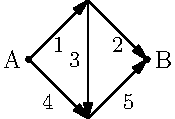
\includegraphics{coop_nefteprovod.pdf}
\end{figure}

Собственники труб и пропускная способность труб в таблице:

\begin{tabular}{|c|c|c|}

\hline 
Номер трубы & Пропускная способность & Владелец \\
\hline
1 & 2 л/час & Андрей \\
2 & 3 л/час & Борис \\
3 & 1 л/час & Володя \\
4 & 2 л/час & Борис \\
5 & 3 л/час & Андрей \\
\hline
\end{tabular}

Потребители нефти готовы платить 1 рубль за скорость передачи 1 литр/час. 

Найдите вектор Шепли.

